%\documentclass[a4paper]{article}
\usepackage[utf8]{inputenc}
\usepackage[spanish, es-tabla, es-noshorthands]{babel}
\usepackage[table,xcdraw]{xcolor}
\usepackage[a4paper, footnotesep=1.25cm, headheight=1.25cm, top=2.54cm, left=2.54cm, bottom=2.54cm, right=2.54cm]{geometry}
%\geometry{showframe}

%\usepackage{wrapfig}			%Wrap figure in text
\usepackage[export]{adjustbox}	%Move images
\usepackage{changepage}			%Move tables

\usepackage{tikz}
\usepackage{amsmath}
\usepackage{amsfonts}
\usepackage{amssymb}
\usepackage{float}
\usepackage{graphicx}
\usepackage{caption}
\usepackage{subcaption}
\usepackage{multicol}
\usepackage{multirow}
\usepackage{wrapfig}
\setlength{\doublerulesep}{\arrayrulewidth}
\usepackage{booktabs}
\usepackage[numbib, nottoc, notlot, notlof]{tocbibind}

\usepackage{hyperref}
\hypersetup{
    colorlinks=true,
    linkcolor=blue,
    filecolor=magenta,      
    urlcolor=blue,
    citecolor=blue,    
}

%Change Font Size

% #1 = size, #2 = text
\newcommand{\setparagraphsize}[2]{{\fontsize{#1}{6}\selectfont#2 \par}}		%Cambia el size de todo el parrafo
\newcommand{\setlinesize}[2]{{\fontsize{#1}{6}\selectfont#2}}				%Cambia el font de una oración

\newcommand{\note}[1]{
	\begin{center}
		\huge{ \textcolor{red}{#1} }
	\end{center}
}

%FONTS (IMPORTANTE): Compilar en XeLaTex o LuaLaTeX
\usepackage{anyfontsize}	%Font size
\usepackage{fontspec}		%Font type

\usepackage{etoolbox}
\usepackage{todonotes}

\newcommand{\observacion}[2]{  \ifnumequal{1}{#1}{ { \todo[inline,backgroundcolor=red!25,bordercolor=red!100]{\textbf{Observación: #2}} } }{  }  }

\setcounter{topnumber}{2}
\setcounter{bottomnumber}{2}
\setcounter{totalnumber}{4}
\renewcommand{\topfraction}{0.85}
\renewcommand{\bottomfraction}{0.85}
\renewcommand{\textfraction}{0.15}
\renewcommand{\floatpagefraction}{0.8}
\renewcommand{\textfraction}{0.1}
\setlength{\floatsep}{5pt plus 2pt minus 2pt}
\setlength{\textfloatsep}{5pt plus 2pt minus 2pt}
\setlength{\intextsep}{5pt plus 2pt minus 2pt}

\newcommand{\quotes}[1]{``#1''}
\usepackage{array}
\newcolumntype{C}[1]{>{\centering\let\newline\\\arraybackslash\hspace{0pt}}m{#1}}
\usepackage[american]{circuitikz}
\usetikzlibrary{calc}
\usepackage{fancyhdr}
\usepackage{units} 

\graphicspath{{../Control de posición no lineal/}{../Control de fuerza no lineal/}{../Control híbrido no lineal/}{../Referencias/}{../Deducción de modelo/}{../Conclusiones/}}

\pagestyle{fancy}
\fancyhf{}
\lhead{22.99 - Automación Industrial}
\rhead{Lambertucci, Londero B., Maselli, Mechoulam}
\rfoot{Página \thepage}

%Items con bullets y no cuadrados
\renewcommand{\labelitemi}{\textbullet }


%\begin{document}

\subsection{Caracterización del problema}
Finalmente se realizó un control híbrido, el cual toma parte tanto del control de posición como de fuerza.

\subsection{Esquema de control propuesto}
El esquema de control propuesto es nuevamente una linealización por realimentación de la siguiente manera:
\begin{figure}[H]
	\centering
	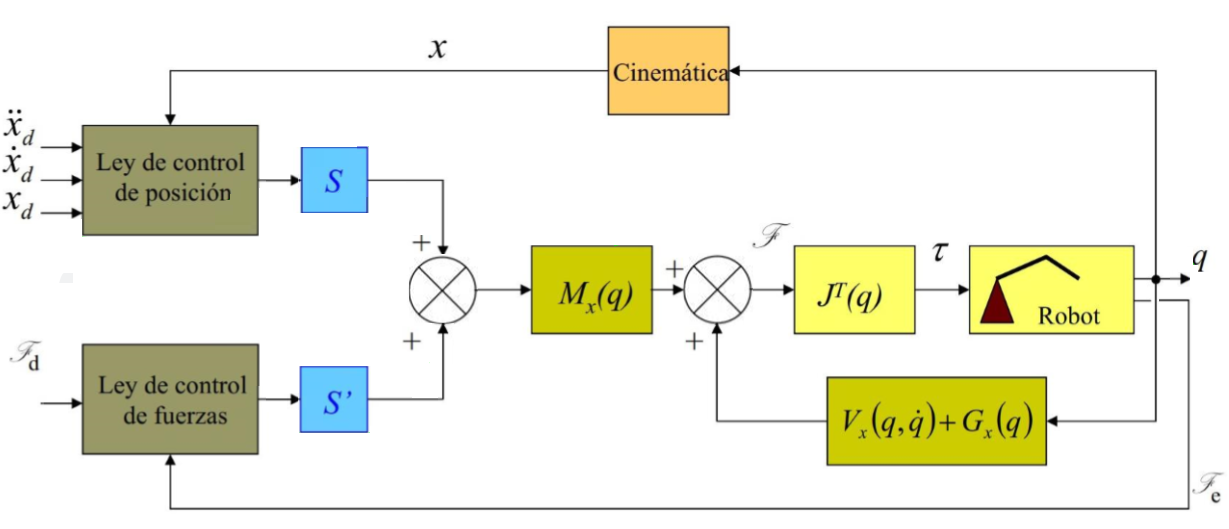
\includegraphics[width=0.8\linewidth]{ImagenesControl híbrido no lineal/controlh}
	\caption{Topología del control de fuerza no lineal.}	
	\label{fig:control_f_modelo_h}
\end{figure}

\observacion{\verObs}{HABLAR DE VALORES DE GANANCIAS}

\subsection{Resultados}
Se realizó el simulink del sistema. Es así que se obtuvieron los gráficos siguientes.

Debido a las ganancias elegidas existe un control más fuerte asociado al control de fuerzas que al de trayectoria. Por dicha razón es que aproximadamente en el segundo 1, el EE se acerca a la pared y sigue pegado a esta.

Si bien se mueve en la dirección provista por el control de posición, lo hace pegado a la pared.
\begin{figure}[H]
	\centering
	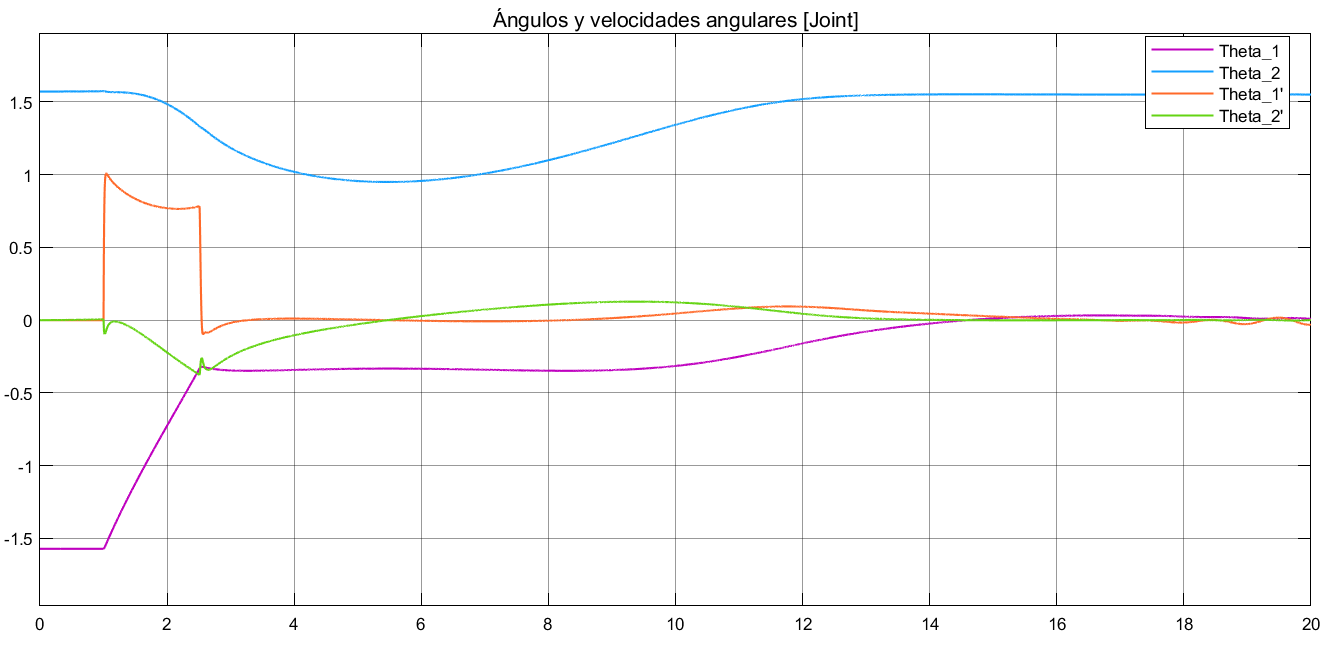
\includegraphics[width=0.8\linewidth]{ImagenesControl híbrido no lineal/3_3_a}
	\caption{Ángulos en función del tiempo en espacio joint.}	
	\label{fig:cthetas}
\end{figure}

Se puede ver como convergen las posiciones del EE con las de la referencia.
\begin{figure}[H]
	\centering
	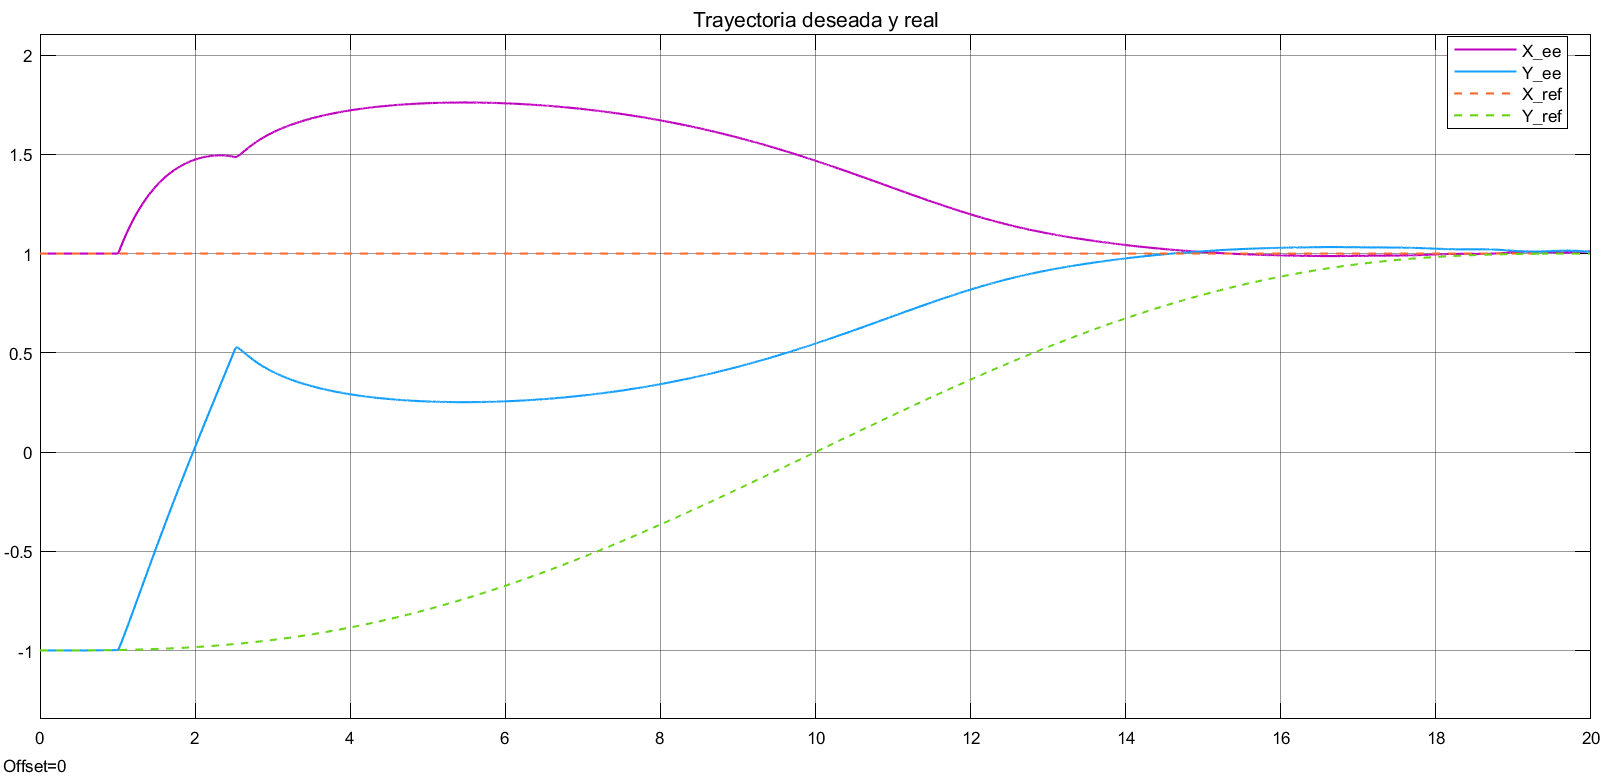
\includegraphics[width=0.8\linewidth]{ImagenesControl híbrido no lineal/3_3_b}
	\caption{Posición  del EE.}	
	\label{fig:cpos}
\end{figure}

En la Figura (\Ref{fig:cxy}) se puede apreciar claramente lo discutido previamente, es decir como el EE, al llegar a la pared, este se pega a ella y avanza sobre la misma en dirección al punto descrito por el control de posición.

\begin{figure}[H]
	\centering
	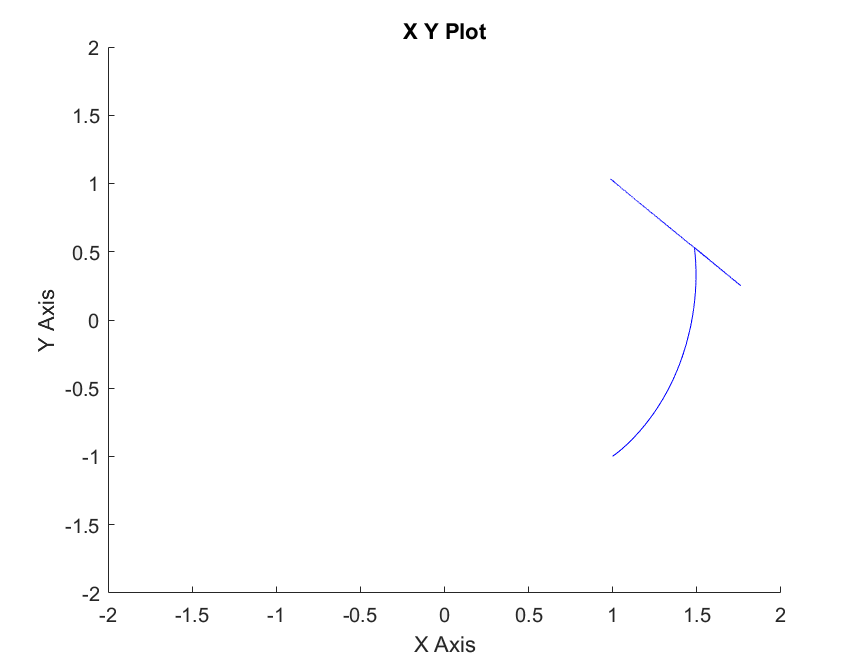
\includegraphics[width=0.5\linewidth]{ImagenesControl híbrido no lineal/3_3_c}
	\caption{Gráfico XY.}	
	\label{fig:cxy}
\end{figure}

Aquí también se ve como aproximadamente en el segundo 2.5 el EE llega a la pared y comienza a hacer fuerza contra la misma. Esta fuerza se mantiene por todo el recorrido hasta el fin.

\begin{figure}[H]
	\centering
	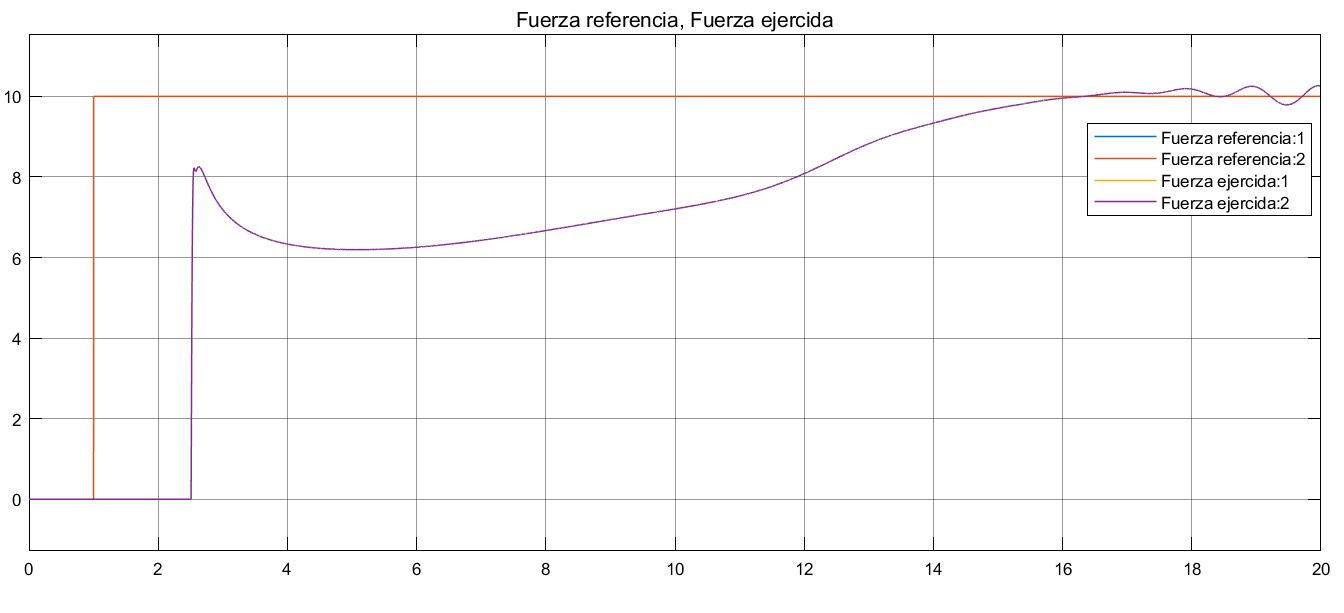
\includegraphics[width=0.8\linewidth]{ImagenesControl híbrido no lineal/3_3_e}
	\caption{Gráfico XY.}	
	\label{fig:cf}
\end{figure}

Ademas se incluyó un disturbio a la planta tanto en posición como en velocidad. En este caso, se optó por hacer el disturbio en el segundo 5. Es así que se observa como reacciona el manipulador en pleno movimiento en vez de en régimen permanente.

Se puede ver que, si bien hay mucho mayor desvío de la posición, las variables convergen. 

\begin{figure}[H]
	\centering
	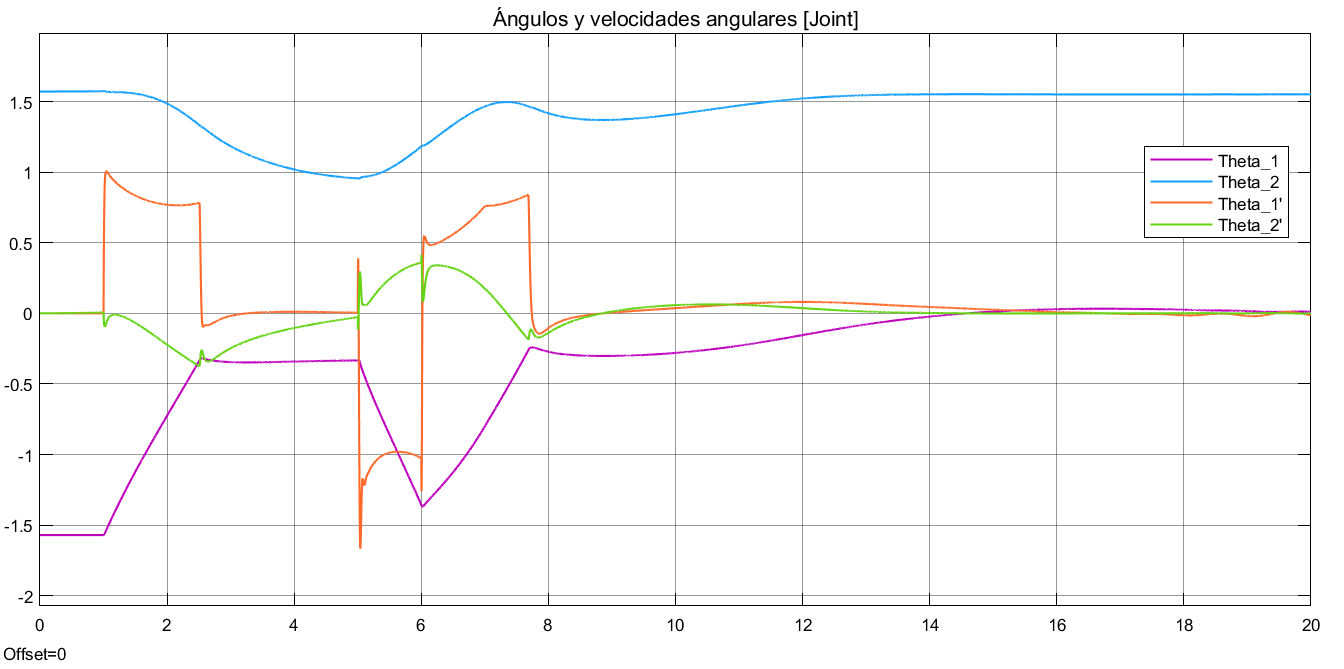
\includegraphics[width=0.8\linewidth]{ImagenesControl híbrido no lineal/3_3_f_a}
	\caption{Ángulos en función del tiempo en espacio joint.}	
	\label{fig:cthetasd}
\end{figure}

En este caso es el control en el que mayor error respecto de la referencia hay.

\begin{figure}[H]
	\centering
	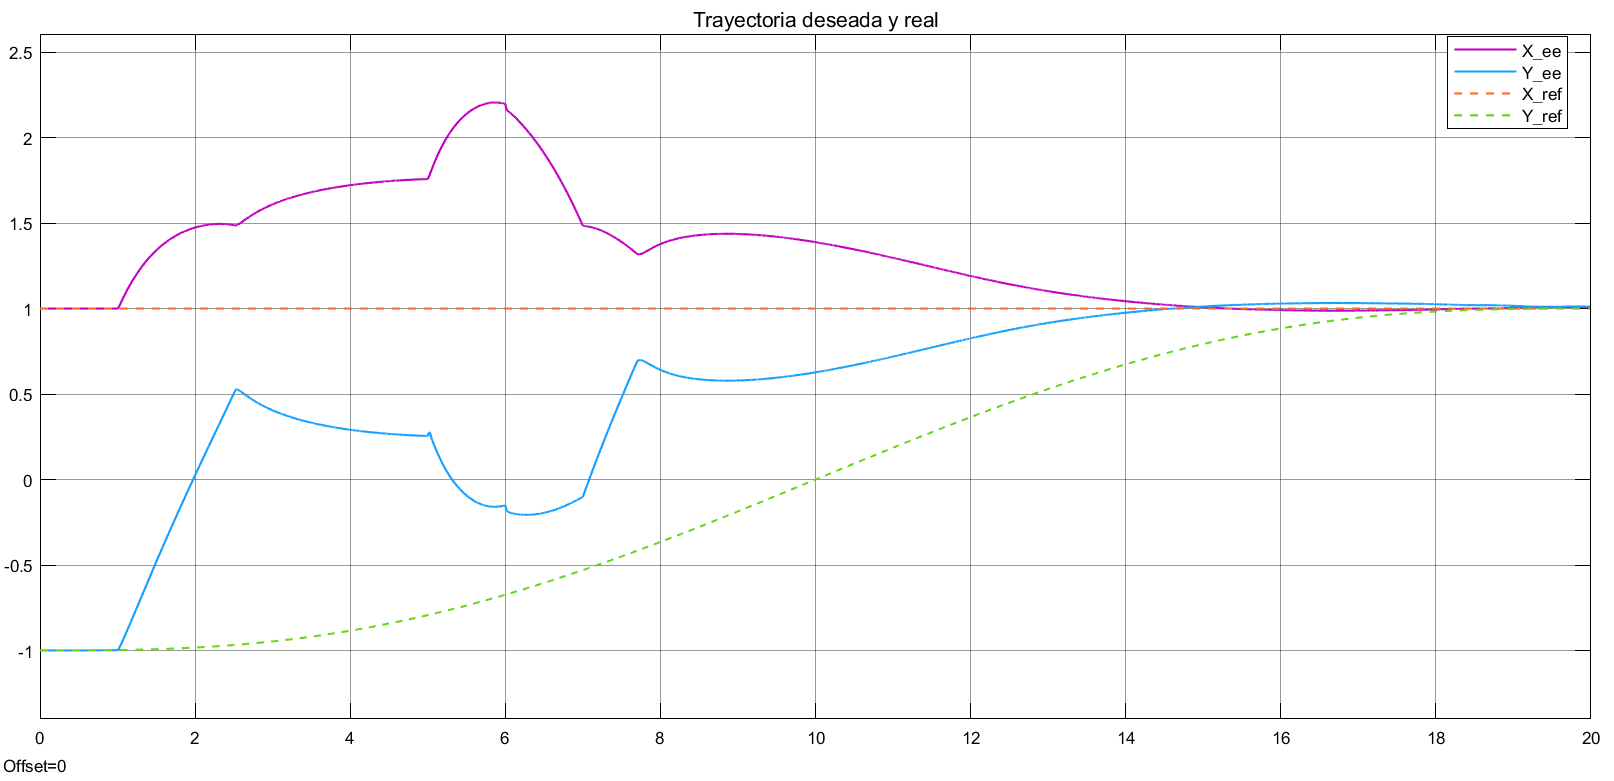
\includegraphics[width=0.8\linewidth]{ImagenesControl híbrido no lineal/3_3_f_b}
	\caption{Posición del EE.}	
	\label{fig:cposd}
\end{figure}

Aquí se puede ver como se desplazó el EE por el plano, pegado a la pared hasta el disturbio.
\begin{figure}[H]
	\centering
	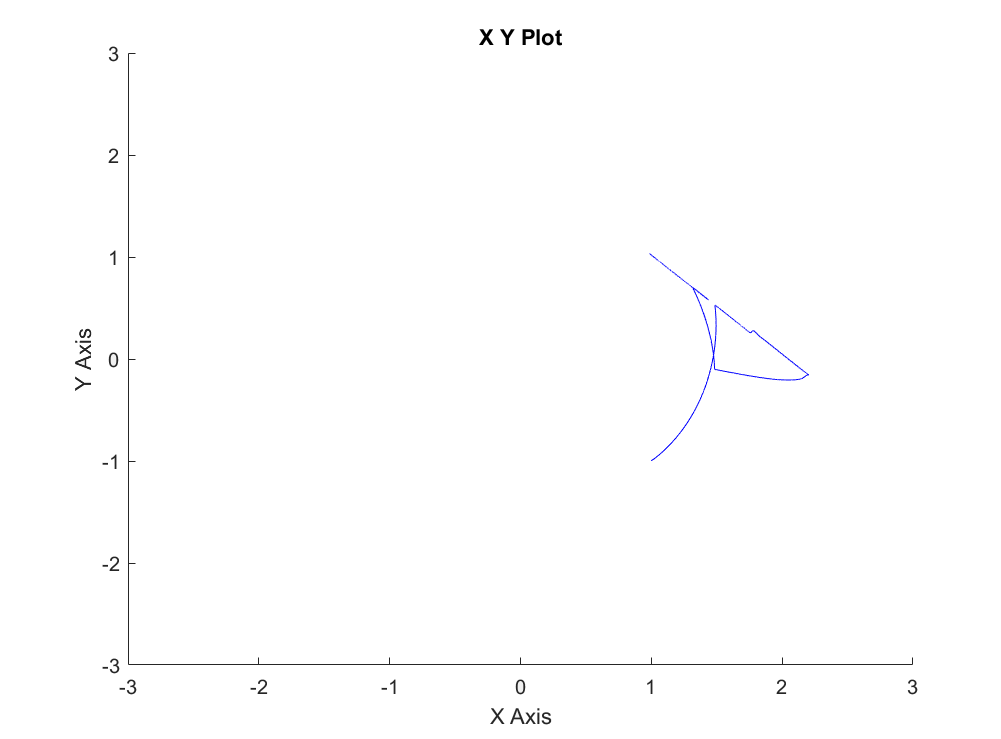
\includegraphics[width=0.5\linewidth]{ImagenesControl híbrido no lineal/3_3_f_c}
	\caption{Gráfico XY.}	
	\label{fig:cxyd}
\end{figure}

En este gráfico es donde mejor se puede ver el disturbio introducido y como rápidamente el control de fuerzas vuelve a su referencia.

\begin{figure}[H]
	\centering
	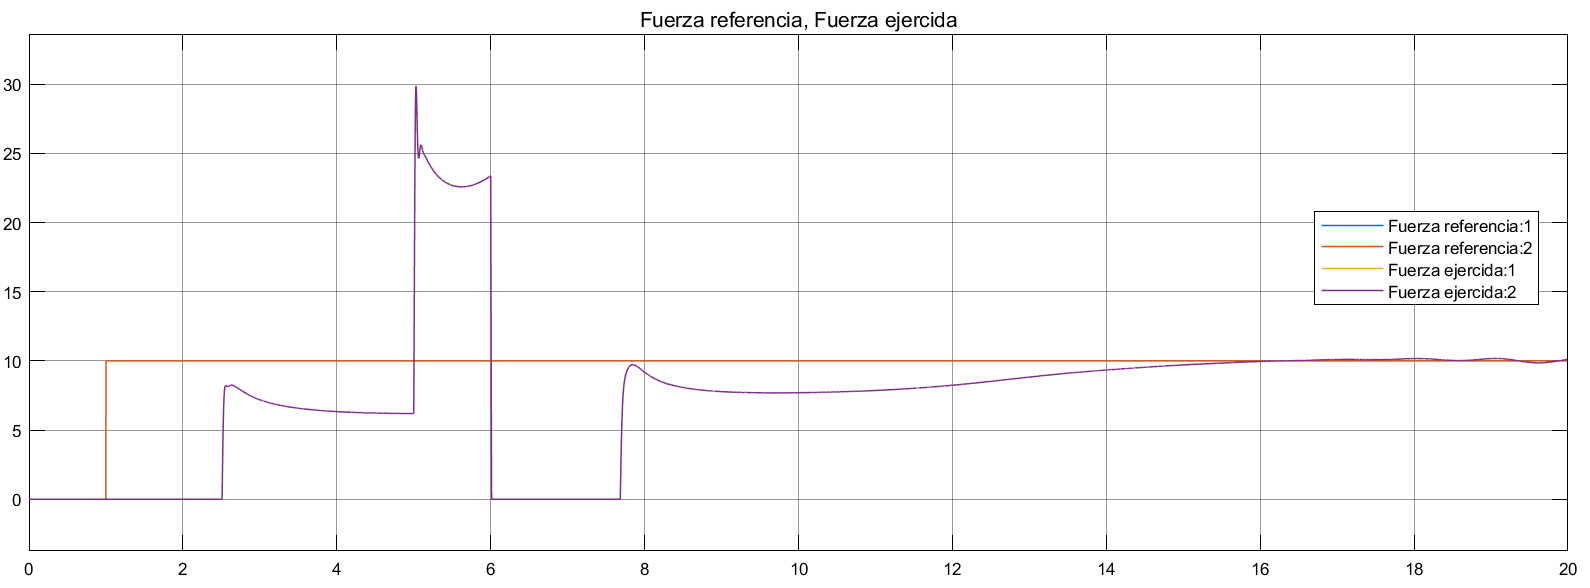
\includegraphics[width=0.8\linewidth]{ImagenesControl híbrido no lineal/3_3_f_e}
	\caption{Fuerza deseada y real.}	
	\label{fig:cfd}
\end{figure}
%\end{document}